\begin{figure}
\centering
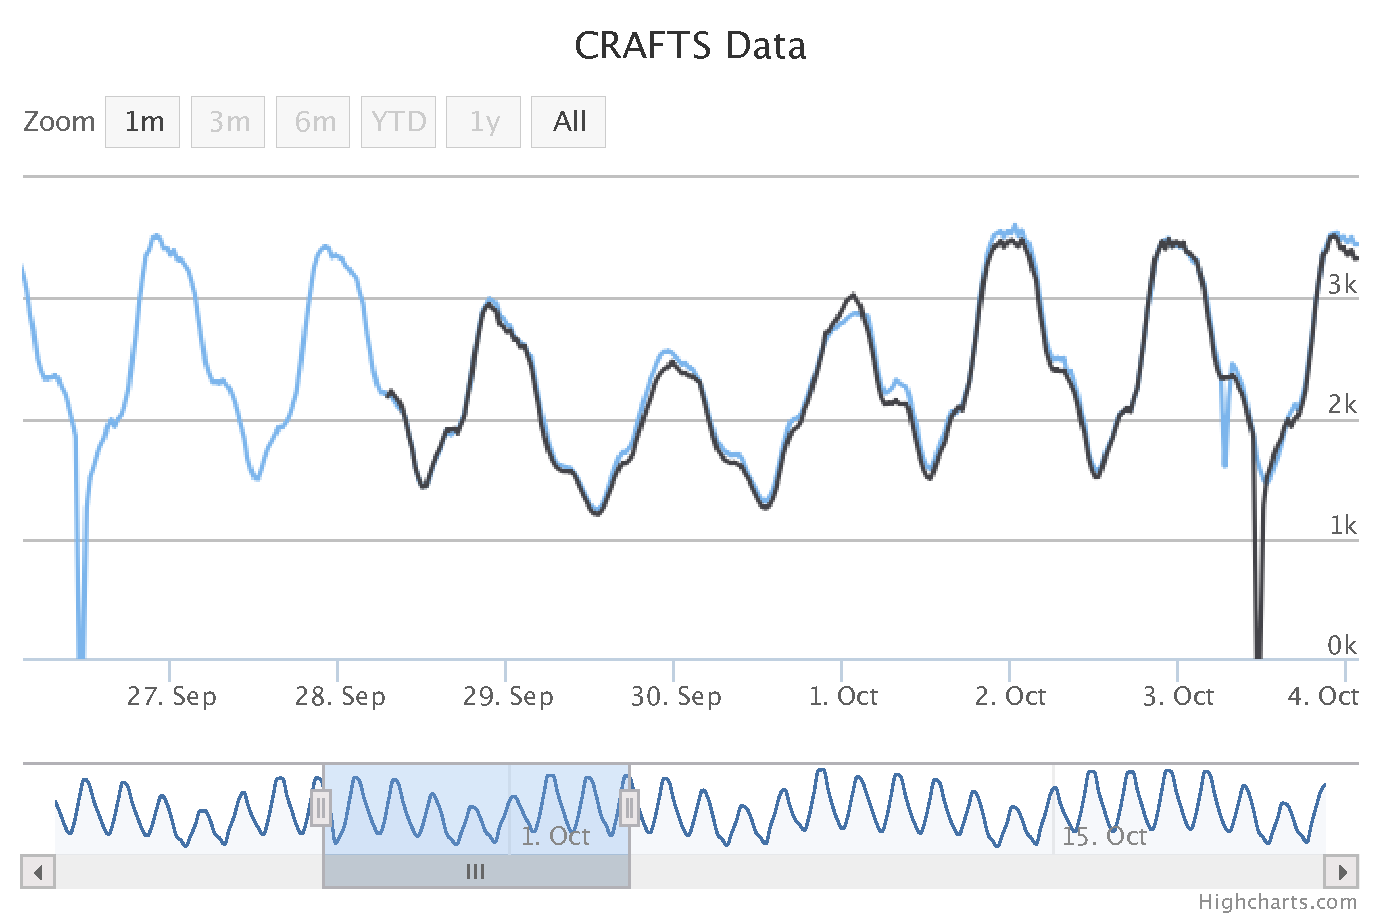
\includegraphics[width=\textwidth]{results/graphs/translation_outage.pdf}
\caption{An outage translated by the translation predictor}
\label{fig:translation_outage}
\end{figure}

\begin{figure}
\centering
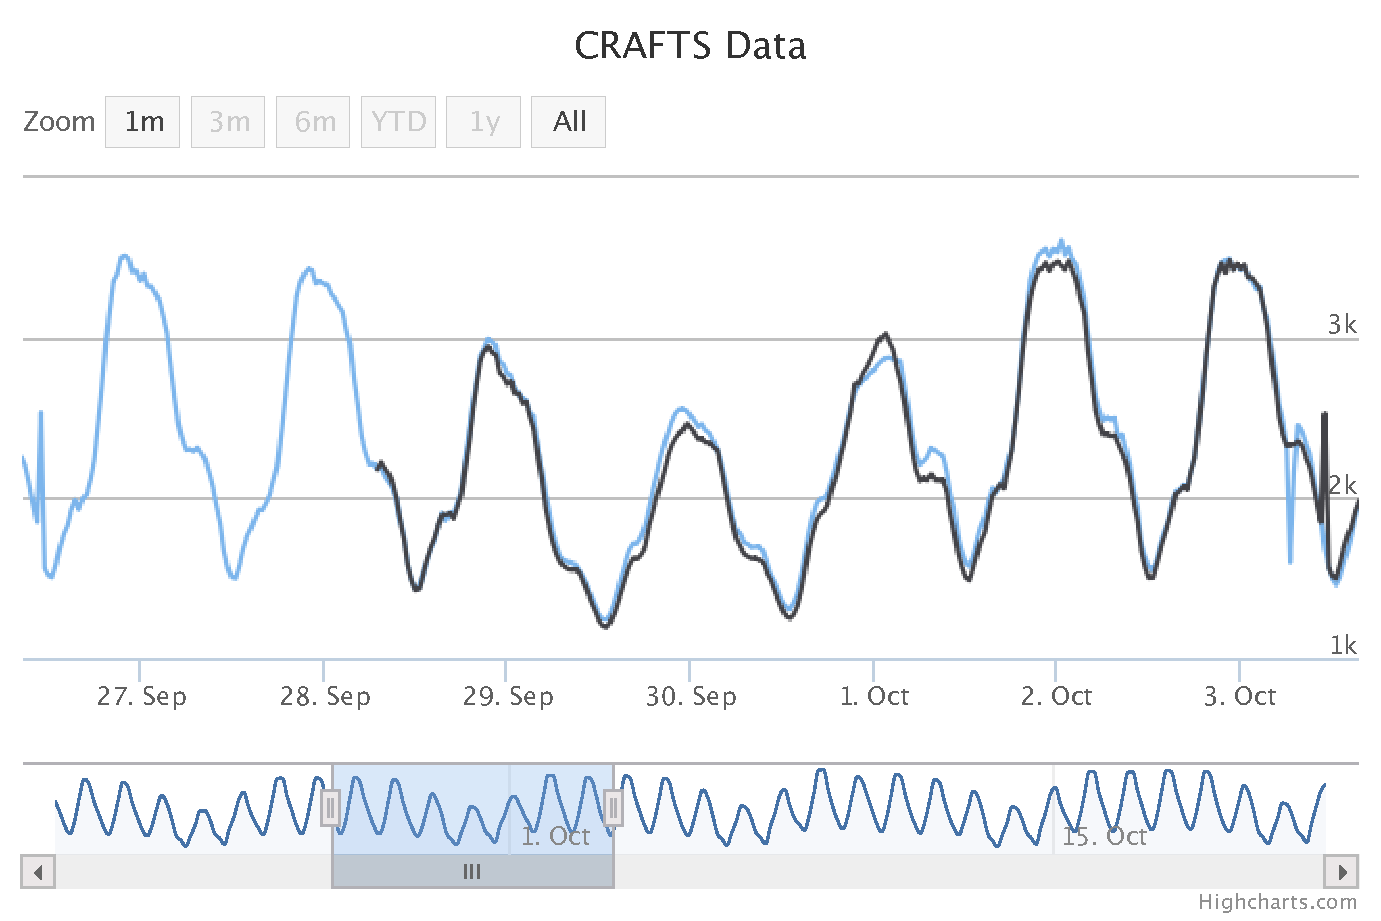
\includegraphics[width=\textwidth]{results/graphs/translation_spike.pdf}
\caption{A usage spike translated by the translation predictor}
\label{fig:translation_spike}
\end{figure}

\begin{table}[H]
\centering
\begin{tabular}{| l | l | l |}
\hline
Type & RMSD & Percent \\ \hline
Under & 113 & 68.7\% \\ \hline
Over & 76 & 31.3\% \\ \hline
Total & 103 & \\ \hline
\end{tabular}
\caption{Translation predictor results for the baseline workload}
\end{table}

% Outage workloads

\begin{table}[H]
\centering
\begin{tabular}{| l | l | l |}
\hline
Type & RMSD & Percent \\ \hline
Under & 122 & 68.7\% \\ \hline
Over & 76 & 31.3\% \\ \hline
Total & 110 & \\ \hline
\end{tabular}
\caption{Translation predictor results for the 10-minute outage workload}
\end{table}

\begin{table}[H]
\centering
\begin{tabular}{| l | l | l |}
\hline
Type & RMSD & Percent \\ \hline
Under & 132 & 68.8\% \\ \hline
Over & 76 & 31.2\% \\ \hline
Total & 117 & \\ \hline
\end{tabular}
\caption{Translation predictor results for the 30-minute outage workload}
\end{table}

\begin{table}[H]
\centering
\begin{tabular}{| l | l | l |}
\hline
Type & RMSD & Percent \\ \hline
Under & 145 & 68.9\% \\ \hline
Over & 76 & 31.1\% \\ \hline
Total & 127 & \\ \hline
\end{tabular}
\caption{Translation predictor results for the 60-minute outage workload}
\end{table}

% Spike workloads

\begin{table}[H]
\centering
\begin{tabular}{| l | l | l |}
\hline
Type & RMSD & Percent \\ \hline
Under & 113 & 68.7\% \\ \hline
Over & 83 & 31.3\% \\ \hline
Total & 105 & \\ \hline
\end{tabular}
\caption{predictor results for the low spike workload}
\end{table}

\begin{table}[H]
\centering
\begin{tabular}{| l | l | l |}
\hline
Type & RMSD & Percent \\ \hline
Under & 113 & 68.7\% \\ \hline
Over & 91 & 31.3\% \\ \hline
Total & 107 & \\ \hline
\end{tabular}
\caption{predictor results for the mid spike workload}
\end{table}

\begin{table}[H]
\centering
\begin{tabular}{| l | l | l |}
\hline
Type & RMSD & Percent \\ \hline
Under & 113 & 68.7\% \\ \hline
Over & 102 & 31.3\% \\ \hline
Total & 110 & \\ \hline
\end{tabular}
\caption{predictor results for the high spike workload}
\end{table}